
    \begin{frame}{Balance}

\begin{proposition} \label{balancedproperty}
Let $\pi$ be a permutation in $\zpx$, then $\pi_v$ is a balanced 
sequence over $\z_v$ if and only if $v \mid p-1$.
\end{proposition}
\begin{proof}
  
      The number of $x \equiv a \mod v$ in $[1,p-1]$ is
      \[  |\pi_v|_a = \lceil (p-1 - ((a-1) \bmod v))/v\rceil\]

  \end{proof}
      \end{frame}


      \begin{frame}{Period}

        \begin{lemma} \label{lemma_near_balanced_period}
If $p \equiv \alpha \neq 1 \Mod v$, then $\pi_v$ has period $N =p-1$ for any $\pi$ permutation of $\zpx$.
\end{lemma}
\begin{proof}

  The difference in the number of occurrences of any two symbols must be a multiple of $(p-1)/N$. But   
  \[
    |\pi_v|_a = \begin{cases} \lceil (p-1)/v \rceil &  0 \leq a < \alpha -1, \\
      \lfloor (p-1)/v \rfloor & \mbox{otherwise}.
    \end{cases}
  \]
\end{proof}

\end{frame}

\begin{frame}{Period}


\begin{theorem}For every $\epsilon >0 $ there exists an $n_{\epsilon}$ so that for 
  all $p \geq n_{\epsilon}$, the number $T$ of balanced sequences $\pi_v$ with period 
  $p-1$ satisfies 
  \begin{equation} \label{T_bound_epsilon}
    (p-1)!(1-\epsilon) \leq T \leq (p-1)!.
  \end{equation}
\end{theorem}
  
\end{frame}


\begin{frame}{Special case}

  When $q$ is prime and $p=vq+1$,
  \[
    \frac{(p-1)! - T}{(p-1)!} = \frac{v!(q!)^v}{(p-1)!} 
    \]

    This includes the case of Sophie Germain primes.
  
  \end{frame}

  \begin{frame}{de Bruijn graph}
    \usetikzlibrary {arrows.meta}
    \begin{center}
      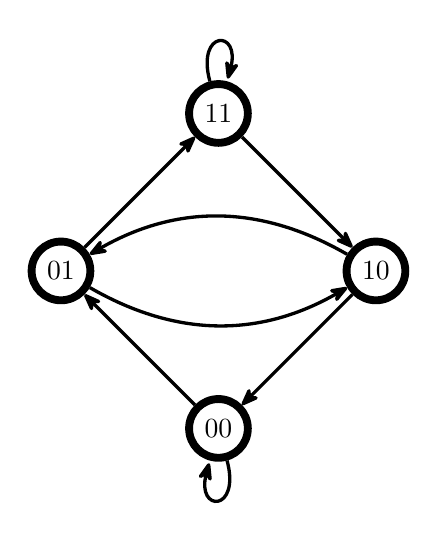
\begin{tikzpicture}
%        [->,>={Stealth[round]},shorten >=1pt,auto,node distance=2.8cm,on grid,semithick]
        [->,>={Stealth[round]},auto,node distance=2.8cm,very thick]
      \node (00) at  (0,0) [circle,draw=black,line width=1.0mm] {00};
      \node (01) at  (-2,2) [circle,draw=black,line width=1.0mm] {01};
      \node (10) at  (2,2) [circle,draw=black,line width=1.0mm] {10};
      \node (11) at  (0,4) [circle,draw=black,line width=1.0mm] {11};

      \path (00) edge [loop below] (00);
      \path (00) edge (01);
      \path (10) edge (00);
      \draw (10) to[out=150,in=30]  (01);
      \draw (01) to[out=-30,in=-150]  (10);
      \path (01) edge (11);
      \path (11) edge (10);
      \path (11) edge [loop above] (11);
    \end{tikzpicture}
    \end{center}

  \end{frame}

  \begin{frame}{Transfer Matrix}


    
    Transfer matrix is directed adjacency matrix of de Bruijn graph with variables
    \[
      T =  \bordermatrix{ & 00 & 01 & 10 & 11 \cr
     00 & ux_0 & ux_0 & 0 & 0 \cr
     01 & 0 & 0 & x_0 & x_0 \cr
     10 & 1 & 1 & 0 & 0\cr
   11 & 0 & 0 & 1 & 1}
      \]

\[
      C =  \bordermatrix{ & 00 & 01 & 10 & 11 \cr
     00 & 1 & 0 & 0 & 0 \cr
     01 & 0 & 1 & 0 & 0 \cr
     10 & 0 & 0 & 1 & 0\cr
   11 & 0 & 0 & 0 & 1}
      \]

\[
  \sum_{\mathbf{k} \in \mathbb{N}^t} a_n({\mathbf k})x^{\mathbf k} = \sum_{z',z'' \in \z_v^t} C_{z',z''} T^{n}_{z',z''}.
\]
      
\end{frame}


\begin{frame}{Asymptotic Normality}

  \begin{theorem}[Bender, Richmond, Williamson 1983] 
Suppose $a_n(k)$ is admissible at 1 for $n \equiv n_0 \Mod d$ and that 
$\Lambda$ is d-dimensional. Then $a_n(k)$ satisfies a central limit theorem 
for $n \equiv n_0 \Mod d$ with means and covariance matrix asymptotically 
proportional to $n$.  Let $q$ be such that $qc \in \Lambda$ for all 
$c \in \z^v$.  Then $a_n(k)$ satisfies a local limit theorem modulo 
$\Lambda$ for $n \equiv n_0 \Mod {dq}$
\end{theorem}
  
\end{frame}

\begin{frame}{Asymptotic Normality}

  \begin{theorem}
Let $z \in \z_v^t$ and $t(\kappa)$ be the number of balanced circular sequences 
of length $n$ over $\z_v$ for which $\lambda(z) = \kappa$. 
There exists a $m_{\lambda},b_{\lambda},c_{\lambda} \in \R$ such that
  \[
    \sup_{\kappa} \left |\frac{\sqrt{2\pi b_{\lambda}}t(\kappa)}{\binom{vl}{l,l,\ldots,l}}-c_{\lambda} e^{(\kappa-m_{\lambda})^2/b_{\lambda}} \right| = o(1). 
  \]
Let $b \in \z_v$, $t \in \N$ and $r(\kappa)$ be the number of balanced circular 
sequences of length $n$ over $\z_v$ for which $\rho(b,t) = \kappa$. 
There exists a $m_{\rho},b_{\rho},c_{\rho} \in \R$ such that
  \[
    \sup_{\kappa} \left |\frac{\sqrt{2\pi b_{\rho}}r(\kappa)}{\binom{vl}{l,l,\ldots,l}}-c_{\rho} e^{(\kappa-m_{\rho}^2)/b_{\rho}} \right | = o(1). 
  \]
\end{theorem}
  
\end{frame}
 	
\begin{frame}{Mean for tuples}
 
\begin{multline*}
  \frac{n}{v^t}\left( 1 + \frac{- (t^2 - 2tv + v^2 - t)(v - 1)}{2n} \right ) +O\left(\frac{1}{n}\right) \\
  \leq  E(\lambda(z)) \leq  \\
  \frac{n}{v^t} \left(1 + \frac{t(v-1)}{2n}\right) +  O\left(\frac{1}{n}\right)
\end{multline*}

  \end{frame}
 	
\begin{frame}{Variance for tuples}
 
  \begin{multline*}
    \frac{n}{v^{2t}} \left( \frac{2v^t}{2} + \frac{-12t^2v^t}{24n} \right) + O\left(\frac{1}{n}\right)\\
    \lesssim    \VAR(\lambda) \lesssim \\
    \frac{n}{v^{2t}} \left( \frac{2v^t(v+1)}{2(v-1)} + \frac{12v^{t+2}t}{24n(v-1)} \right) + O\left(\frac{1}{n}\right)
\end{multline*}
  \end{frame}


 	
\begin{frame}{Runs}

\begin{align*}
     E(\rho(b,t)) &= \frac{(l(v-1)-1)(v-1)l(l)_t}{(n-1)_{t+1}}, \\   
  \VAR(\rho(b,t)) &= \frac{(l(v-1)-1)(v-1)l(l)_t}{(n-1)_{t+1}} \\
    & + \frac{(v-1)l(l)_{2t}(l(v-1)-1)^2(l(v-1)-2)}{(n-1)_{2t+2}} \\
    & - \left(\frac{(l(v-1)-1)(v-1)l(l)_t}{(n-1)_{t+1}}\right)^2 .
\end{align*}
Where $l = n/v$.
\end{frame}  


	
\begin{frame}{Runs}

\begin{align*}
E(\rho(b,t)) &= \frac{n(v-1)}{v^{t+2}} \left((v-1) 
               - \frac{(v-1)^2t^{2} -(v+3)(v-1)t +2}{2n}\right) \\
  &\qquad + O\left (\frac{1}{n}\right)\\
  \VAR(\rho(b,t)) &\approx \frac{n(v-1)^2}{v^{t+2}} \left(1 
     + \frac{-(v-1)t^2}{2n}\right) + O\left(\frac{1}{n}\right)
\end{align*}



\end{frame} 

%%% Local Variables:
%%% TeX-master: "../main.tex"
%%% End:
